\section{Механизм взаимодействия сервера сбора данных с УСПД}
\setcounter{figure}{0}

В разрабатываемой системе сервер является инициатором всех обменов данными, а клиенты ожидают запроса для передачи данных. Схема взаимодействия приведена на рисунке \ref{scheme2:scheme2}.

\begin{figure}[h!]
 \center{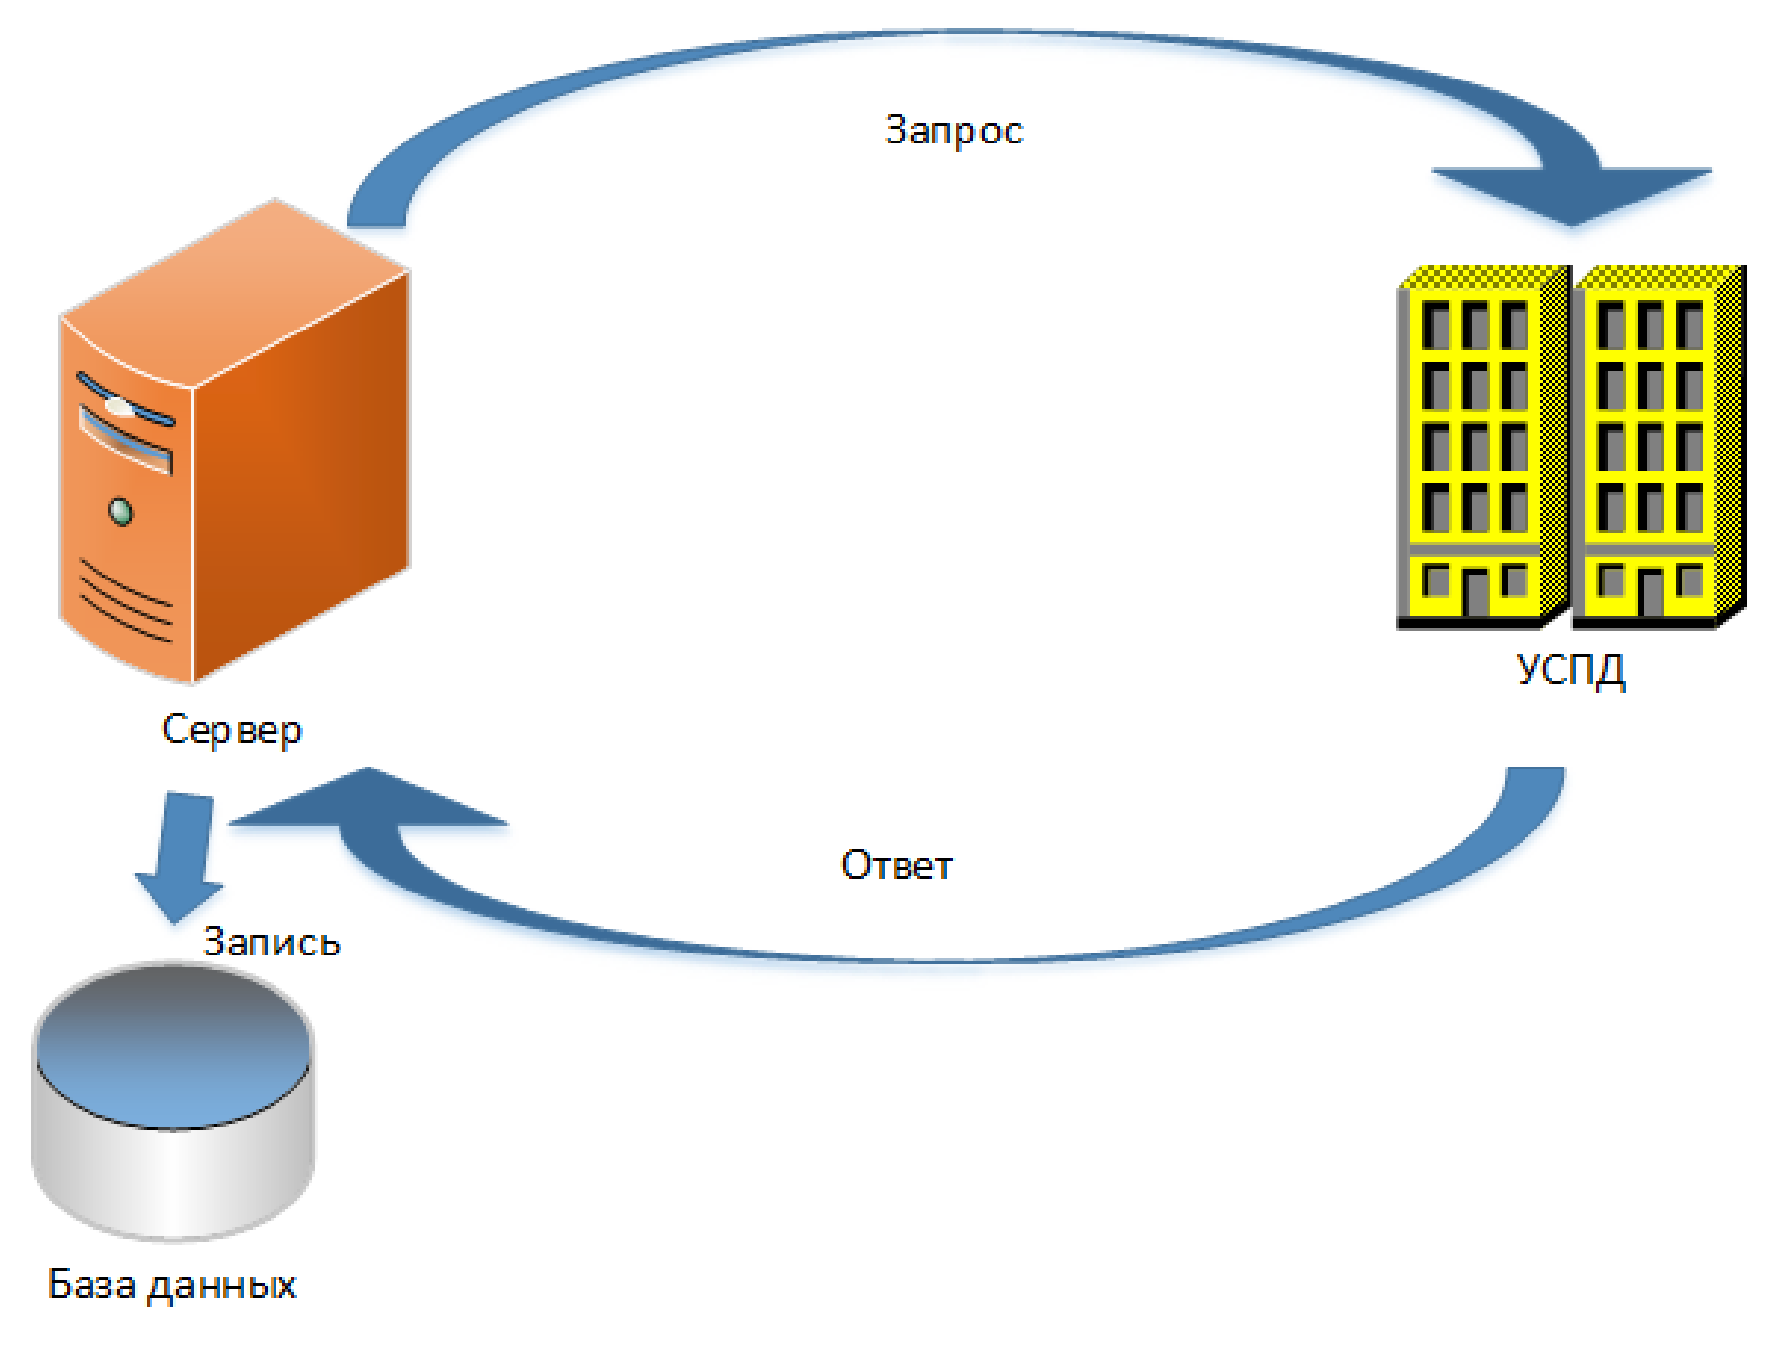
\includegraphics[width=0.8\linewidth]{scheme2}}
 \caption{Схема взаимодействия сервера с УСПД}
 \label{scheme2:scheme2}
\end{figure}

Данный механиз позволяет реализовать опрос УСПД по списку, хранящемуся на сервере, что исключит возможность отправки данных с несанкционированных устройств. Так же появляется возможность обнаружения неисправности УСПД либо ошибки сети, на который сервер будет реагировать предупреждениями. 

Данные, полученные с УСПД, записываются во временную базу данных для последующей обработки и отправки на центральный сервер. В этой же базе данных хранится список всех УСПД, подконтрольных данному серверу. Схема представлена на рисунке \ref{scheme3:scheme3}.

\begin{figure}[h!]
 \center{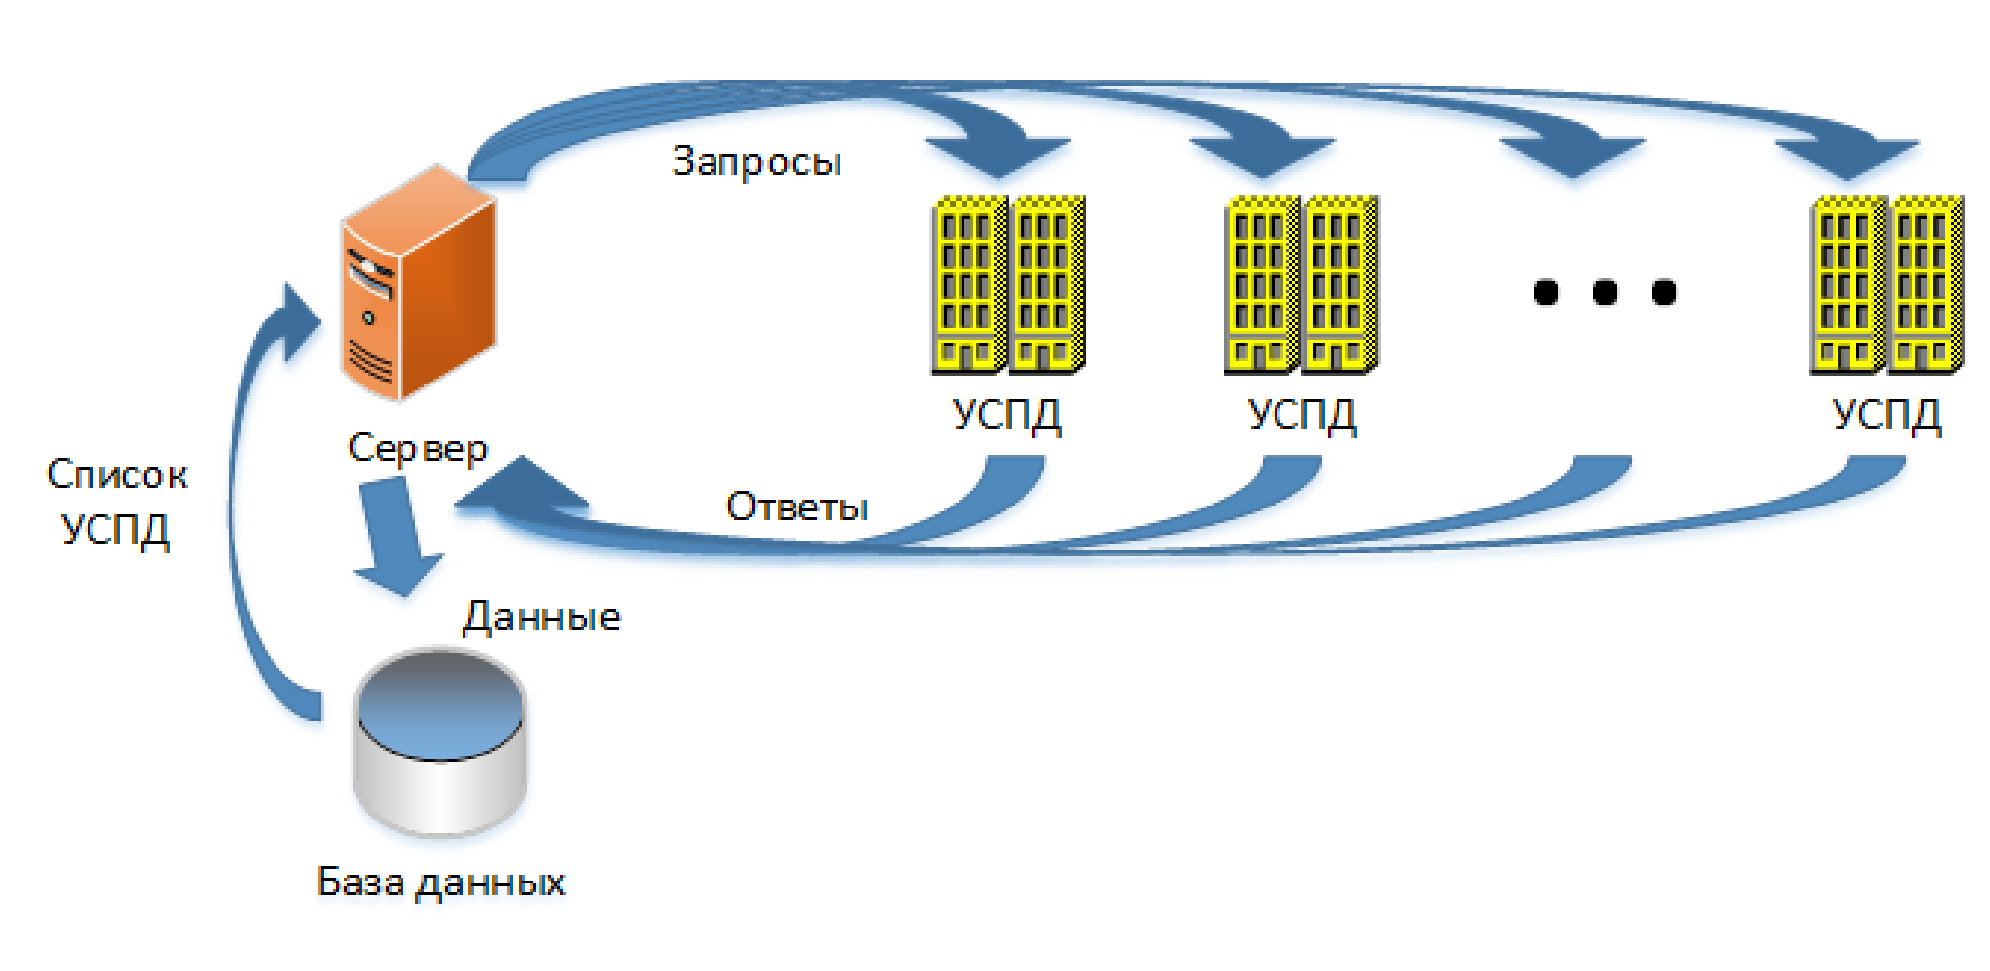
\includegraphics[width=0.8\linewidth]{scheme3}}
 \caption{Механизм взаимодействия с группой УСПД}
 \label{scheme3:scheme3}
\end{figure}
